\chapter{Overview}

\section{History}

Analytical models for predicting fire behavior have been evolving since the 1960s. Over the
past decade, the completeness of the models has grown considerably. In the beginning, the focus
of these efforts was to describe in mathematical language the various phenomena which were
observed in fire growth and spread. These separate representations have typically described only
a small part of a fire. However, when combined they can create a complex computational model
that can predict the expected course of a fire.

Once a mathematical representation of the underlying physics has been developed, the conservation
equations can be re-cast into predictive equations for temperature, smoke and gas
concentration and other parameters of interest, and solved numerically.
The equations are usually in the form of differential equations. A complete set of equations can
describe the conditions produced by the fire at a given time in a specified volume of air.
Referred to as a control volume, the model assumes that the predicted conditions within this
volume are uniform at any time. Thus, the control volume has one temperature, smoke density,
gas concentration, etc. Different models divide the building into different numbers of control
volumes depending on the desired level of detail. The most common fire model, known as a
zone model, generally uses two control volumes to describe a compartment � an upper layer and
a lower layer. In the compartment with the fire, additional control volumes for the fire plume or
the ceiling jet may be included to improve the accuracy of the prediction (see figure \ref{fig:Zone_Terms}).

\begin{figure}
\begin{center}
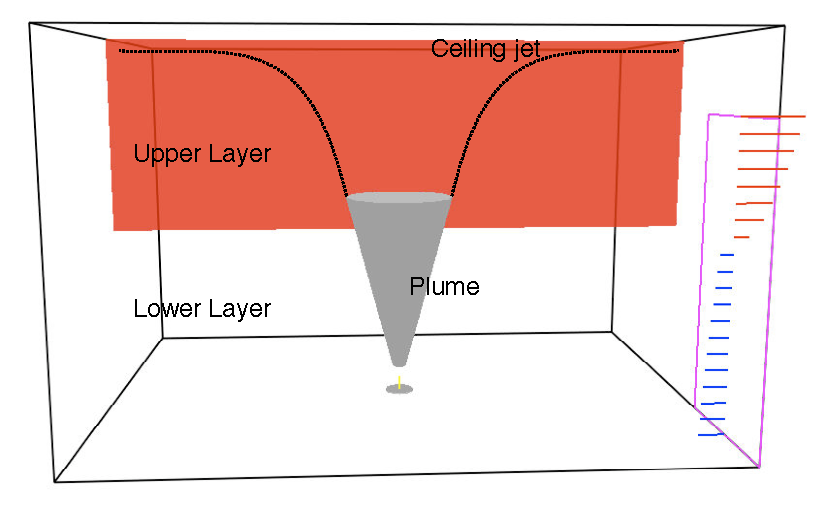
\includegraphics[width=4.0in]{FIGURES/Overview/Zone_Terms}\\
\end{center}
\caption{Zone Model Terms.}
 \label{fig:Zone_Terms}
\end{figure}

This two-layer approach has evolved from observation of such layering in real-scale fire experiments.  Hot gases collect at the ceiling and fill the compartment from the top.  While these experiments show some variation in conditions within the layer, these are small compared to the differences between the layers.  Thus, the zone model can produce a fairly realistic simulation under many common and important conditions.

Other types of models include network models and field models.  Network models use one control volume per compartment and are used to predict conditions in spaces far removed from the fire compartment where temperatures are near ambient and layering does not occur.  The field model goes to the other extreme, dividing the compartment into thousands or millions of control volumes.  Such models can predict the variation in conditions within the layers, but typically require far longer run times than zone models.  They are used when a highly detailed prediction of the flow itself is of interest.

\section{Model Evaluation}

The process of model evaluation is critical to establishing both the acceptable uses and limitations of fire models. It is not possible to evaluate a model in total; instead, available guides such as ASTM E1355 \cite{ASTM:E1355} are intended to provide a methodology for evaluating the predictive capabilities for a specific use . Validation for one application or scenario does not imply validation for different scenarios. Several alternatives are provided for performing the evaluation process including comparison of predictions against standard fire tests, full-scale fire experiments, field experience, published literature, or previously evaluated models.

The use of fire models currently extends beyond the fire research laboratory and into the engineering, fire service and legal communities. Sufficient evaluation of fire models is necessary to ensure that those using the models can judge the adequacy of the scientific and technical basis for the models, select models appropriate for a desired use, and understand the level of confidence which can be placed on the results predicted by the models. Adequate evaluation will help prevent the unintentional misuse of fire models. Verification is a process to check the correctness of the solution of the governing equations.  Verification does not imply that the governing equations are appropriate; only that the equations are being implemented and solved correctly. Validation is a process to determine the appropriateness of the governing equations as a mathematical model of the physical phenomena of interest.  Typically, validation involves comparing model results with experimental measurement.  Differences that cannot be explained by numerical errors in the model or uncertainty in the experiments are attributed to the assumptions and simplifications of the physical model. These terms are used together to perform a model assessment. The more general term, �model assessment,� encompasses both verification and validation of a computer model.

In general, this document follows the ASTM E1355 \cite{ASTM:E1355} guide for model assessment and provides a model assessment for the zone fire model CFAST.  The guide provides four areas of evaluation for predictive fire models:

\begin{itemize}
\item Defining the model and scenarios for which the evaluation is to be conducted (chapter 2),
\item Assessing the appropriateness of the theoretical basis and assumptions used in the model (chapter 3),
\item Assessing the mathematical and numerical robustness of the model (chapter 4), and
\item Quantifying the uncertainty and accuracy of the model results in predicting the course of events in similar fire scenarios (chapters 5 and 6).
\end{itemize}